\documentclass[a4paper,10pt]{article} % type, taille police

\usepackage[utf8]{inputenc} % encodage
\usepackage[T1]{fontenc} % encodage
\usepackage[french]{babel} % gestion du français
\usepackage{amssymb} % symboles mathématiques
\usepackage{textcomp} % flèche,  intervalle
\usepackage{stmaryrd} % intervalle entiers

\usepackage[left=3cm,right=3cm,top=3cm,bottom=3cm]{geometry} % marges
\usepackage[hidelinks]{hyperref} % sommaire interactif dans un pdf
\usepackage[nottoc, notlof, notlot]{tocbibind} % affichage des références dans la table des matières (?)
\usepackage{float} % placement des figures
\usepackage[toc,page]{appendix} % ajout d'annexes
\usepackage{amsthm} % format des déf, prop...
\usepackage{amsmath} % matrices, ...
\usepackage{multirow} % fusionner cellules verticalement

\usepackage{tikz} % affichage de schémas
\usepackage{graphicx} % affichage d'images
\usepackage{url} % inclure des urls
\usepackage{bbold} % fonction caractéristique 1

\renewcommand{\appendixtocname}{Annexes} % renommage annexes
\renewcommand{\appendixpagename}{Annexes}

\definecolor{bgreen}{rgb}{0.30,0.70,0}

\theoremstyle{definition} % pas d'italique pour le format des déf, prop...
\newtheorem{thm}{Théorème} % \begin{thm} \end{thm}
\newtheorem{cor}[thm]{Corollaire}
\newtheorem{defi}[thm]{Définition}
\newtheorem{ex}[thm]{Exemple}
\newtheorem{lem}[thm]{Lemme}
\newtheorem{rem}[thm]{Remarque}
\newtheorem{conj}[thm]{Conjecture}

\newcommand{\R}{\mathbb{R}}
\newcommand{\Q}{\mathbb{Q}}
\newcommand{\N}{\mathbb{N}}
\newcommand{\Z}{\mathbb{Z}}

%#############################################################################################################%
%#############################################################################################################%
%#############################################################################################################%

\title{Reconnaissance et indexation de formes}
\author{Quentin Cormier \and Yassine Hamoudi}
\date{4 mai 2015}

\begin{document}

\maketitle

\tableofcontents

%#############################################################################################################%
%#############################################################################################################%
%#############################################################################################################%

\section{Introduction}

Il existe de nombreuses manières de caractériser une image en vue de reconnaître l'objet qu'elle représente. Cependant, la plupart des descripteurs ``élémentaires'' (périmètre de l'image, nombre de composantes connexes, surface ...) sont peu efficaces individuellement et nécessitent d'être combinés astucieusement pour donner de bons résultats.

Nous avons recherché un moyen robuste et plus concis de classifier en 70 catégories le millier d'images du projet. Notre méthode consiste à étudier la propagation d'une onde à l'intérieur d'une image. En effet, cette propagation dépend directement de la forme de l'objet. De la même manière que deux tambours de forme circulaire renvoient des sons proches, deux images de pommes devraient propager les ondes de façon similaires. Par ailleurs, cette méthode semble insensible à de nombreuses perturbations (rotation, translation, dilatation...).

Notre travail s'inspire de \cite{Zuliani04} et \cite{KhabouHR07}. Nous étudierons dans un premier temps quels descripteurs peuvent être construits à partir du problème de la propagation d'une onde dans une image. Nous chercherons également la métrique la plus appropriée pour comparer deux vecteurs descripteurs associés à deux images. La résistance de notre algorithme à différentes perturbations (rotation, bruit...) sera également vérifiée théoriquement et expérimentalement.

\section{Méthode}

L'objectif est de classifier plusieurs images en noir et blanc dans une catégorie parmi 70 possibles.
On dispose pour cela d'une dizaine d'images "d'entraînement" par catégories (le \textit{training set}, noté $\mathcal{T}$).

A partir de ces images d'entrainement on doit pouvoir classifier une image inconnue dans l'une des catégories.

Au vu de la taille relativement restreinte du \textit{training set}, on décide d'encoder l'image en un vecteur de réels (le \textit{descripteur} associé à l'image), et d'utiliser 
une distance entre deux descripteurs pour classifier une image inconnue.

Ainsi, pour une image inconnue $M$, on calcule le descripteur associé $d_M$, puis on cherche l'image la plus proche dans le \textit{training set} : $$M' = argmin_{M' \in \mathcal{T}}{d(d_M, d_{M'})}_,   $$ $d$ étant la distance entre descripteurs choisie.

On prédit alors la classe de $M$ comme étant celle de $M'$.


\subsection{Descripteur associé à l'image}

La partie principale du projet consiste donc à calculer un descripteur associé à chaque image. Ce vecteur de réels doit dépendre de la forme de l'image. Idéalement, deux images ayant des formes similaires doivent donner deux descripteurs similaires.

Dans la mesure du possible, il doit être également invariant par translation, par rotation et par dilatation : translater une image, la tourner, l'agrandir ou la rétrécir ne change pas la catégorie de l'image, et donc ne devrait pas changer le descripteur. On aimerait également avoir une robustesse au bruit.

On choisit ici d'utiliser un descripteur inspiré par la physique qui respecte ces différentes contraintes.

\subsection*{Onde associée à un domaine}

En physique, il est bien connu qu'une onde stationnaire se propageant dans une cavité ne peut se propager seulement en certaines fréquences discrètes qui dépendent de la forme de la cavité.
On se propose de construire un descripteur basé sur ces fréquences. On comprends bien qu'il sera facile de garantir l'invariance par rotation et translation : tourner ou bouger la cavité ne change pas les fréquences qui peuvent se propager dans ladite cavité !

Une onde se propageant dans une cavité vérifie l'équation suivante : $$\Delta E + \frac{1}{v^2} \frac{\partial^2 E}{\partial t^2} = 0$$ avec par exemple : $E(x,y,t)$ nulle sur les bords de la cavité (condition aux limites de Dirichlet).

Si l'on recherche les solutions stationnaires, on pose $E = f(x,y)e^{iwt}$, et on obtient : 
\begin{equation}
\left\{ 
  \begin{array}{l}
 \Delta f  - \frac{w^2}{v^2} f = 0 \\
 f  \text{ s'annulant sur les bords de la cavité.} 
   \end{array} \right.
 \label{eigen}
 \end{equation}

Ainsi, on peut voir $f$ comme un vecteur propre de l'opérateur Laplacien et $\frac{w^2}{v^2}$ la valeur propre associée.

\subsection*{Calcul du descripteur}

\subsubsection*{Calcul des valeurs propres du Laplacien d'une image}

Pour calculer effectivement les valeurs propres du Laplacien dans le domaine définit par l'image, on "encode" l'image de taille $N = n*n$ dans un vecteur de taille $n^2$.
On construit alors la matrice de l'opérateur Laplacien discrétisé $\Delta^*$ suivant, de taille N*N: 
$$
\Delta^* =
 \begin{pmatrix}
  -A_n & I_n & \cdots & 0 \\
  I_n & -A_n & \ddots &   \vdots \\
  \vdots  & \ddots  & \ddots & I_n  \\
  0 & \cdots  & I_n & -A_n
 \end{pmatrix}
$$

avec $$A_n =  
\begin{pmatrix}
  -4 & 1 & \cdots & 0 \\
  1  & -4 & \ddots &   \vdots \\
  \vdots  & \ddots  & \ddots & 1  \\
  0 & \cdots  & 1 & -4
 \end{pmatrix}  $$

Puis on multiplie chaque ligne $i+Nj$, $i \in \{1, ..., n\}, j \in \{1, ..., n\}$ de $\Delta^*$ par 0 ou 1, suivant la valeur du pixel $M(i,j)$. On obtient alors une nouvelle matrice $\Delta^*_M$, toujours de taille $N*N$, qui vérifie pour tout vecteur $E$ de taille $N$ : 

\[ (\Delta^*_M E)(x,y) = \left\{ 
  \begin{array}{l l}
    (\Delta^* E)(x,y) & \quad \text{lorsque }(x,y) \text{ est dans le domaine définit par l'image}\\
    0 & \quad \text{sinon}
  \end{array} \right.\]
  
  
  Ainsi, si $E$ vecteur de taille $N$ est un vecteur propre de $\Delta^*_M$ associé à la valeur propre $\lambda$, on a : 
  
  \[ (\Delta^*_M E)(x,y) = \left\{ 
  \begin{array}{l l}
    \lambda E(x,y) & \quad \text{lorsque }(x,y) \text{ est dans le domaine définit par l'image}\\
    0 & \quad \text{sinon}
  \end{array} \right.\]
  
 Donc $E$ est bien une solution de l'équation discrétisée \eqref{eigen} : $E$ correspond à une onde stationnaire associée à la valeur propre $\lambda$ pour le domaine définit par l'image.
  
  On peut généraliser facilement cela pour des images rectangulaires de taille $N = h*w$.
  
  On est donc ramené à calculer les valeurs propres d'une matrice creuse. On utilise la fonction \texttt{numpy.linalg.eigvals} pour trouver effectivement les valeurs propres recherchées.
  
  
  \subsubsection*{Calcul du descripteur associé aux valeurs propres}


A partir du spectre trié par ordre croissant $\{\lambda_0, \lambda_1, ...\}$ calculé précédemment, on construit de manière similaire à \cite{Zuliani04} et \cite{KhabouHR07} deux familles de descripteurs : 
\begin{itemize}
\item Descripteur de type 1 : $\{\frac{\lambda_0}{\lambda_1}, \frac{\lambda_0}{\lambda_2}, \frac{\lambda_0}{\lambda_3}, ... \}$
\item Descripteur de type 2 $\{\frac{\lambda_0}{\lambda_1}, \frac{\lambda_1}{\lambda_2}, \frac{\lambda_2}{\lambda_3},...\}$
\end{itemize}

Le choix du descripteur et sa taille (ainsi que la métrique à utiliser pour comparer les descripteurs) seront discutés dans la partie suivante, à partir de résultats expérimentaux.

\subsection{Normalisation des images}

Avant de calculer les valeurs propres associées à une image, on applique à cette dernière quelques opérations de normalisations.

Tout d'abord, on recadre l'image jusqu'à ce que chaque bord contienne au moins un pixel blanc.

Ensuite, on redimensionne l'image de sorte que le maximum de la largeur et de la hauteur soit de 50 pixels. Cette opérations permet de se ramener à des images de taille au plus $N = 50*50 = 2500$. En effet, on est emmené par la suite à calculer les valeurs propres d'une matrice de taille $N*N$, cette opération est relativement coûteuse en temps de calcul (environ 30s pour $N = 2500$).

Enfin on rajoute un cadre noir autour de l'image, ceci permet de fermer la cavité définie par le motif de l'image.

Exemple:

\begin{center}
  \begin{tabular}{c c c}
     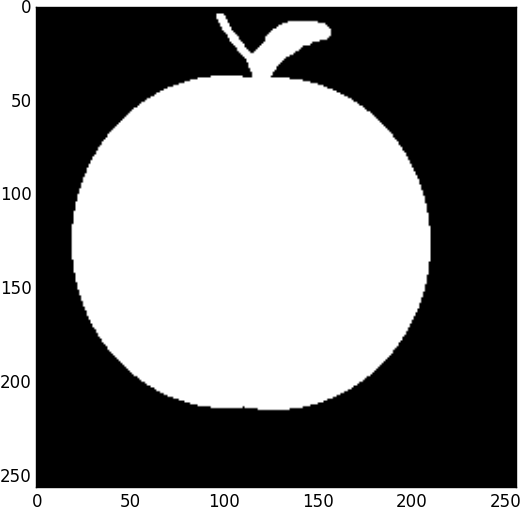
\includegraphics[scale=0.25]{pictures/apple.png} & 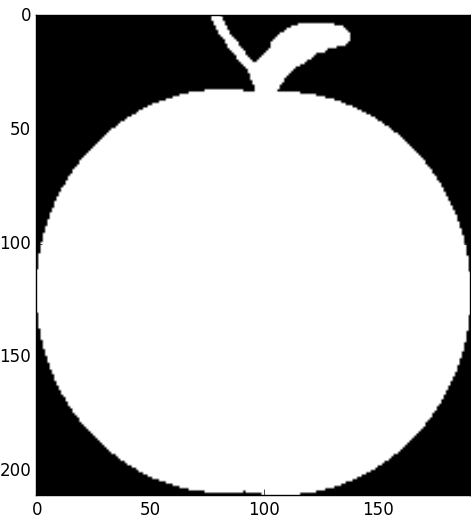
\includegraphics[scale=0.25]{pictures/apple-crop.png} & 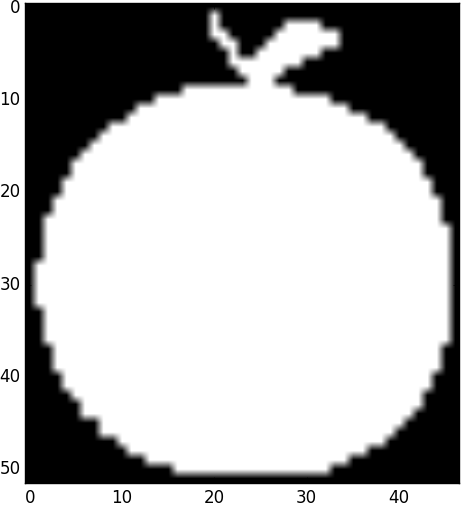
\includegraphics[scale=0.25]{pictures/apple-normalize.png} \\
    Image initiale & Bords rognés & Image après redimensionnement  \\
                          &                        &  et ajout du cadre noir
      \end{tabular}
\end{center}


% mettre des exemples d'images après normalisation

%#############################################################################################################%
%#############################################################################################################%
%#############################################################################################################%

\section{Résultats}

Nous exposons les résultats obtenus grâce à la méthode détaillée précédemment. Nous allons étudier dans un premier temps la sensibilité de notre algorithme aux perturbations (rotation, redimensionnement, bruit, ...), puis nous détaillerons les résultats de classification sur le dataset d'images.

%-------------------------------------------------------------------------------------------------------------%

  \subsection{Sensibilité aux perturbations}

Les valeurs propres du Laplacien de Dirichlet vérifient un certain nombre de propriétés mathématiques qui garantissent que notre descripteur est insensible au redimensionnement, à la rotation et à la translation. Nous vérifions expérimentalement ces propriétés ci-dessous.

~\\
\underline{Redimensionnement} Etant donné un domaine $\Omega$ et un facteur $a > 0$, on a $\lambda_k(a \Omega) = \frac{\lambda_k(\Omega)}{a^2}$ (voir \cite{KhabouHR07}). Or, notre descripteur utilise des rapports de valeurs propres, il est donc inchangé par redimensionnement : $\frac{\lambda_k(a \Omega)}{\lambda_m(a \Omega)} = \frac{\lambda_k(\Omega)}{\lambda_m(\Omega)}$. Nous avons calculé différents rapports pour l'image \texttt{camel-1.pgm}, les résultats figurent table \ref{scale}. Les variations d'une image à l'autre peuvent s'expliquer par les dégrations des contours suite au redimensionnement. Les rapports restent tout de même très proches. En pratique, nous utilisons une longueur de 50 pixels afin d'obtenir des temps de calcul raisonnables (environ 20s pour calculer les valeurs propres associées à une image de taille 50x50).

\begin{table}[H]
  \begin{center}
    \begin{tabular}{l | c c c c c c}
                & $\lambda_1 / \lambda_2$ & $\lambda_1 / \lambda_3$ & $\lambda_1 / \lambda_4$ & $\lambda_2 / \lambda_3$ & $\lambda_3 / \lambda_4$ & $\lambda_4 / \lambda_5$ \\ \hline
      75 pixels & 0.63 & 0.42 & 0.36 & 0.67 & 0.84 & 0.89 \\
      50 pixels & 0.61 & 0.42 & 0.32 & 0.68 & 0.83 & 0.89 \\
      25 pixels & 0.53 & 0.39 & 0.31 & 0.73 & 0.80 & 0.81
    \end{tabular}
  \end{center}
\caption{Rapports de valeurs propres en fonctions de la longueur de l'image \texttt{camel-1.pgm} redimensionnée (l'image initiale est de taille 346x346)}
\label{scale}
\end{table}

~\\
\underline{Translation} Nous recadrons systématiquement l'image afin de conserver le plus petit rectangle contenant la figure. Ceci nous permet d'être insensible aux translations.

~\\
\underline{Rotation} Il a été démontré mathématiquement que les valeurs propres sont inchangées lorsque le domaine subit une rotation (voir \cite{Zuliani04}). Ce résultat se vérifie facilement à partir de quatre rotations appliquées sur \texttt{deer-20.pgm}. Les valeurs propres associées à chaque figure sont regroupées dans la table \ref{rot}.

\begin{center}
  \begin{tabular}{c c c c}
    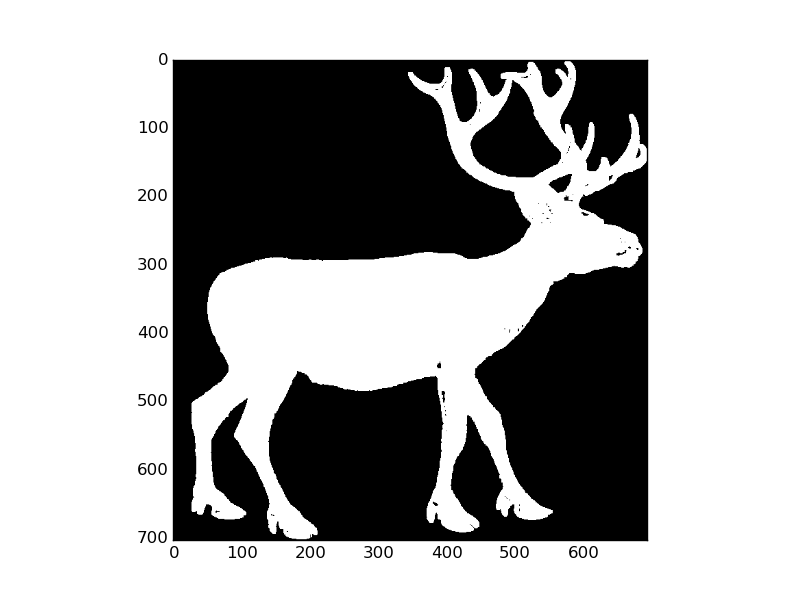
\includegraphics[scale=0.15]{rotate/0.png} & 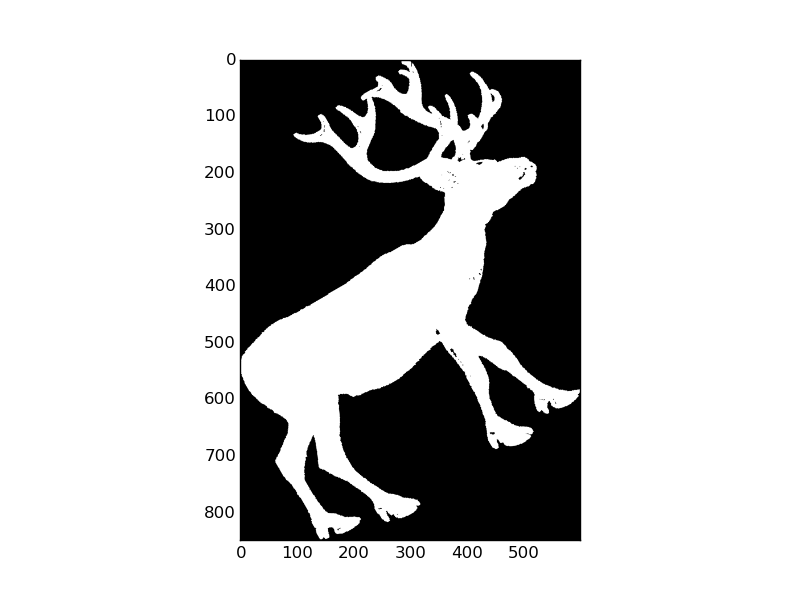
\includegraphics[scale=0.15]{rotate/30.png} & 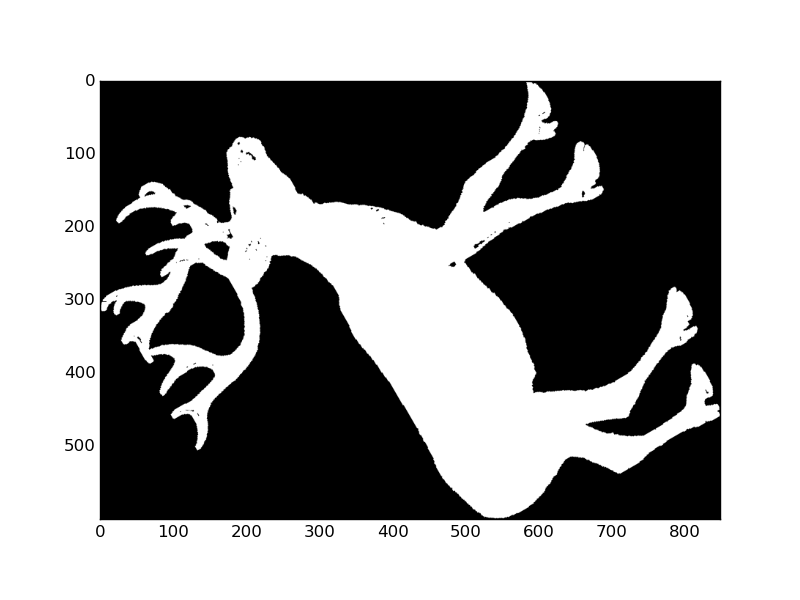
\includegraphics[scale=0.15]{rotate/120.png} & 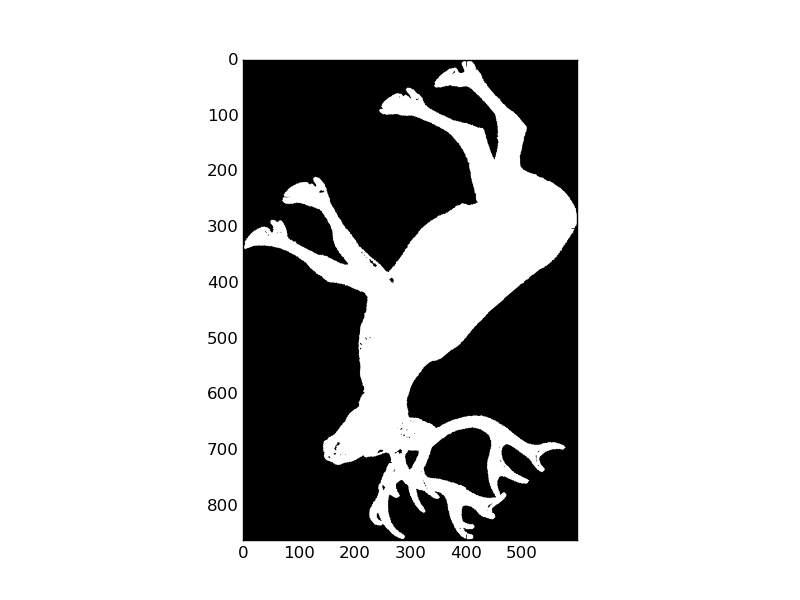
\includegraphics[scale=0.15]{rotate/220.png} \\
    0 degré & 30 degrés & 120 degrés & 220 degrés
  \end{tabular}
\end{center}

\begin{table}[H]
  \begin{center}
    \begin{tabular}{c | c c c c c c c c}
                & $\lambda_1$ & $\lambda_2$ & $\lambda_3$ & $\lambda_4$ & $\lambda_5$ & $\lambda_6$ & $\lambda_7$ & $\lambda_8$ \\ \hline
      0 degré    & 118.57 & 177.16 & 252.35 & 285.53 & 361.22 & 404.89 & 420.69 & 489.36 \\
      30 degrés  & 120.28 & 182.75 & 257.54 & 297.97 & 370.39 & 413.53 & 426.99 & 472.08 \\
      120 degrés & 120.29 & 182.88 & 266.09 & 308.13 & 372.66 & 414.83 & 428.60 & 472.21 \\
      220 degrés & 120.42 & 182.95 & 250.94 & 299.81 & 366.01 & 406.55 & 424.32 & 478.39 
    \end{tabular}
  \end{center}
  \caption{Valeurs propres associées à \texttt{deer-20.pgm} en fonctions de l'angle de rotation}
  \label{rot}
\end{table}

~\\
\underline{Bruit} Le bruit peut déformer le domaine de l'image et modifier par conséquent les valeurs propres. Cependant, les premières valeurs propres ($\lambda_1, \lambda_2, \lambda_3, \dots$) correspondent à la fondamentale et aux premières harmoniques, et donc aux composantes de la solution au Laplacien de Dirichlet de longueur d'onde élevée. Par conséquent, on peut s'attendre à ce qu'une déformation relativement faible du contour impacte peu ces valeurs (contrairement aux valeurs associées à des longueurs d'onde faibles). {\huge \textcolor{red}{Vrai ?}} Par ailleurs, le redimensionnement systématique de l'image que l'on applique permet de gommer partiellement le bruit.

Afin de tester la robustesse au bruit, nous avons implémenté un modèle de bruit de Kanungo (pour un facteur de bruit $0 \leq a \leq 1$, tout point $x$ du domaine à distance $d$ du bord est colorié en noir avec probabilité $a^d$). La table \ref{bruit} démontre le faible impact du bruit sur les valeurs propres.

\begin{center}
  \begin{tabular}{c c c c}
    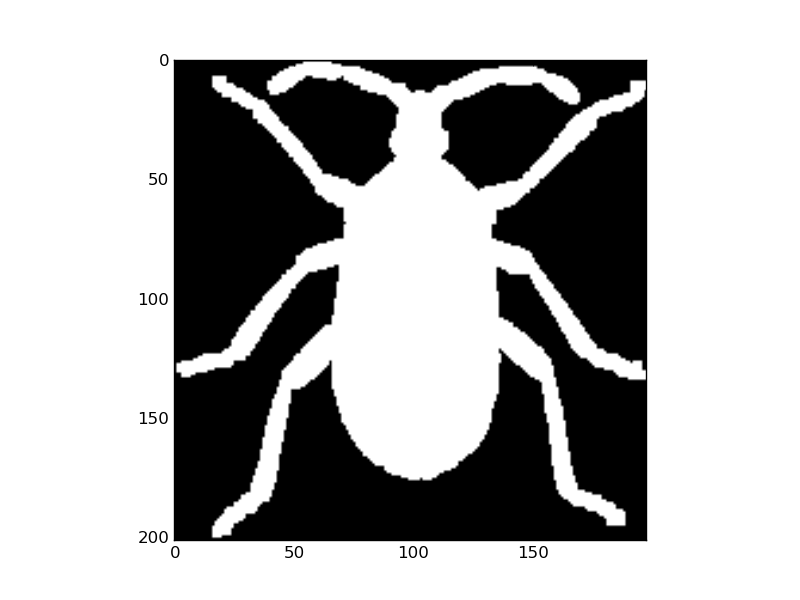
\includegraphics[scale=0.15]{noise/0.png} & 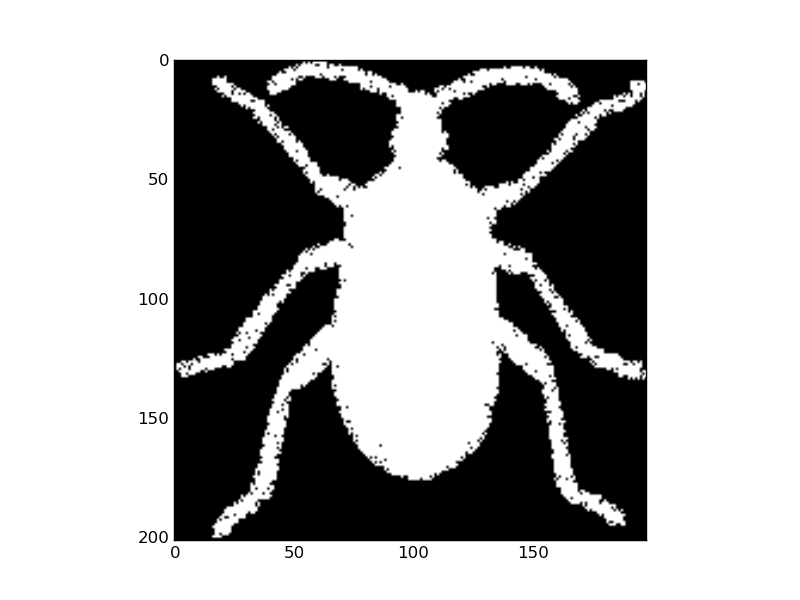
\includegraphics[scale=0.15]{noise/0_3.png} & 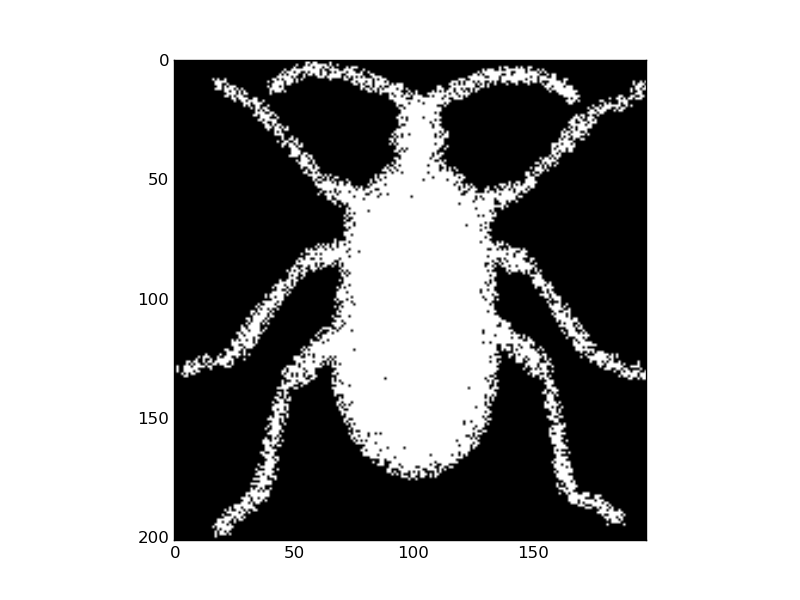
\includegraphics[scale=0.15]{noise/0_6.png} & 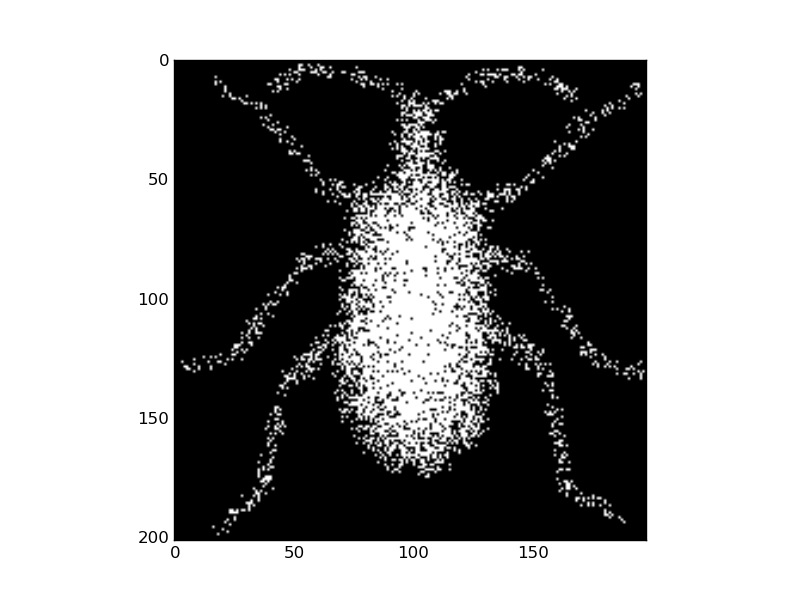
\includegraphics[scale=0.15]{noise/0_9.png} \\
    Bruit 0 & Bruit 0.3 & Bruit 0.6 & Bruit 0.9
  \end{tabular}
\end{center}

\begin{table}[H]
  \begin{center}
    \begin{tabular}{c | c c c c c c c c}
                 & $\lambda_1$ & $\lambda_2$ & $\lambda_3$ & $\lambda_4$ & $\lambda_5$ & $\lambda_6$ & $\lambda_7$ & $\lambda_8$ \\ \hline
      Bruit 0    & 83.93 & 153.41 & 258.76 & 263.10 & 353.64 & 378.19 & 495.73 & 500.11 \\
      Bruit 0.3  & 84.20 & 154.12 & 259.27 & 264.12 & 354.84 & 379.19 & 498.19 & 504.15 \\
      Bruit 0.6  & 84.42 & 155.22 & 262.05 & 264.96 & 355.90 & 388.19 & 503.35 & 514.37 \\
      Bruit 0.9  & 87.02 & 157.19 & 264.77 & 276.22 & 363.54 & 388.21 & 506.28 & 522.61  
    \end{tabular}
  \end{center}
  \caption{Valeurs propres associées à \texttt{beetle-13.pgm} en fonctions du facteur de bruit}
  \label{bruit}
\end{table}

%-------------------------------------------------------------------------------------------------------------%

  \subsection{Performances}

Nous avons testé notre algorithme avec 4 métriques différentes pour mesurer la distance entre descripteurs : 
\begin{itemize}
  \item Distance euclidienne : $d(x,y) = \sqrt{\sum_{i=1}^n (x_i-y_i)^2}$.
  \item Distance de Minkowski (facteur 10) : $d(x,y) = \left(\sum_{i=1}^n (x_i-y_i)^{10}\right)^{1/10}$.
  \item Distance euclidienne carrée (sqeuclidean) : $d(x,y) = \sum_{i=1}^n (x_i-y_i)^2$.
  \item Distance cosine : $d(x,y) = 1 - \frac{\sum_{i=1}^n (x_i-y_i)^2}{\lVert x \rVert_2 \lVert y \rVert_2}$.
\end{itemize}

Nous avons utilisé des descripteurs de type 1 ($\lambda_1/\lambda_2, \lambda_1/\lambda_3, \lambda_1/\lambda_4, \dots$), de type 2 ($\lambda_1/\lambda_2, \lambda_2/\lambda_3,$ $\lambda_3/\lambda_4, \dots$), et un mélange des 2 types.

Etant donné un descripteur (de taille fixée) et une distance, nous avons séparé les 1050 images en deux catégories : un train set (composé d'environ 80\% des images) et un test set (constitué des images restantes). Pour chaque image du test set nous avons recherché l'image du train set qui minimise la distance utilisée. L'algorithme de classification réussit si les deux images appartiennent à la même catégorie.

Nous avons répété 20 fois l'expérience précédente (parallélisée sur 4 coeurs) afin d'obtenir des écarts types inférieurs à 0.03. Les pourcentages de réussites sont regroupés figure \ref{d1} pour le descripteur 1 et figure \ref{d2} pour le descripteur 2. La figure \ref{d3} illustre les performances lorsque le descripteur est composé en partie du type 1 et du type 2 (par exemple l'abscisse 30/10 correspond à un descripteur de taille 40 dont les 30 premières composantes sont de type 1 et les 10 dernières de type 2). Nous avons utilisé uniquement la métrique cosine pour ce dernier test.

\begin{figure}[H]
  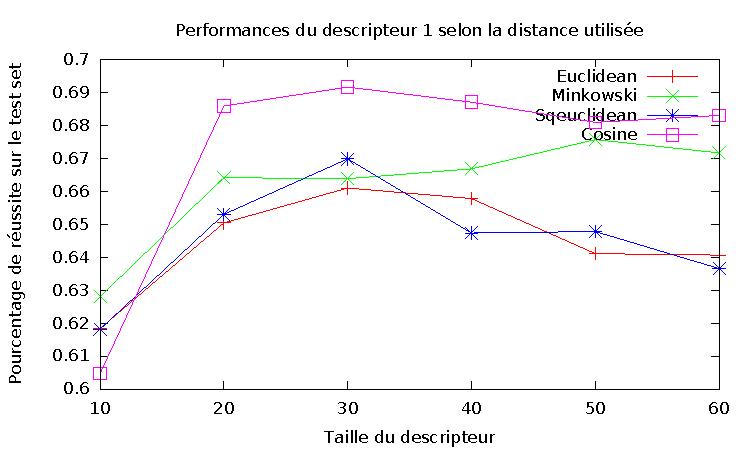
\includegraphics[scale=1.15]{../plot/courbe1.pdf}
\caption{Performances du descripteur 1 selon la distance utilisée}
\label{d1}
\end{figure}

\begin{figure}[H]
  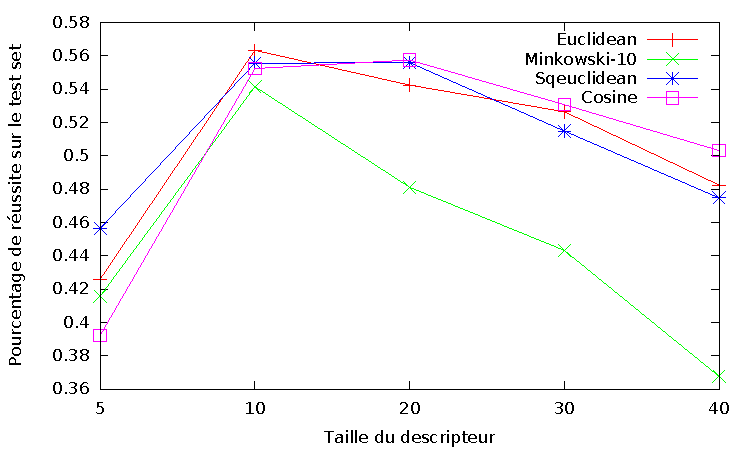
\includegraphics[scale=1.15]{../plot/courbe2.pdf}
\caption{Performances du descripteur 2 selon la distance utilisée}
\label{d2}
\end{figure}

\begin{figure}[H]
  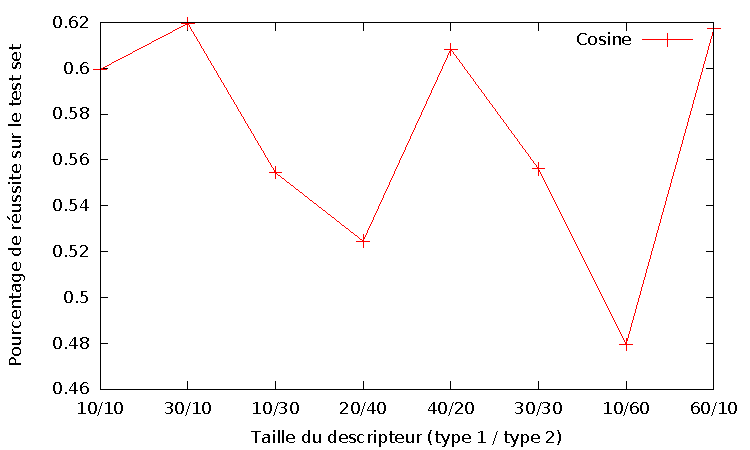
\includegraphics[scale=1.15]{../plot/courbe3.pdf}
\caption{Performances des descripteurs 1 et 2 mélangés, selon la distance utilisée}
\label{d3}
\end{figure}

%#############################################################################################################%
%#############################################################################################################%
%#############################################################################################################%

\section{Discussion}

Le descripteur de type 1 ($\lambda_1/\lambda_2, \lambda_1/\lambda_3, \lambda_1/\lambda_4, \dots$) se révèle être le plus efficace. En effet, comme on peut le constater figure \ref{d1}, quelle que soit la métrique utilisée il permet de dépasser les 60\% de réussite, alors que le descripteur de type 2 (figure \ref{d2}) ne franchit pas 56\%. Mélanger les deux descripteurs ne permet pas non plus d'augmenter les performances comme l'illustre la figure \ref{d3}.

Le meilleur score est obtenu avec la métrique cosine pour un descripteur de type 1 de taille 30 (environ 70\% de réussite). Nous utilisons ces caractéristiques dans notre algorithme final.

Par ailleurs, la faible sensibilité aux perturbations (rotation, dilatation, bruit...) confirme notre hypothèse de départ : lorsque le domaine de l'image est faiblement changé, la propagation des ondes est peu impactée.

Afin d'améliorer la classification, plusieurs paramètres de l'algorithmes pourraient être étudiés plus en détail. Ainsi, on constate que le choix de la métrique est important (pour un descripteur fixé, les performances peuvent changer de 20\% d'une métrique à l'autre). Une approche par machine learning pourrait permettre par exemple de pondérer chaque composante du descripteur (peut-être faut-il donner d'avantage d'importance à $\lambda_1/\lambda_2$ qu'à $\lambda_1/\lambda_3$).


%#############################################################################################################%
%#############################################################################################################%
%#############################################################################################################%

\section{Conclusion}

Reconnaître la forme d'un objet à partir du son qu'il émet est un problème mathématique ancien (voir \cite{kac1966can}). Bien qu'il existe des objets différents émettant des sons identiques (la figure \ref{drum} en est un exemple), dans la majorité des cas le bruit émis est une bonne caractéristique de l'objet.

Comme on a pu le constater dans ce projet, utiliser la propagation d'une onde (via les valeurs propres du Laplacien de Dirichlet) comme seul descripteur permet d'obtenir un outil de classification atteignant 70\% de réussite. Un des atoûts principaux de cette méthode est sa résistance aux perturbations (rotation, bruit...). Par ailleurs, de nombreuses améliorations semblent possibles pour améliorer les performances (choix d'une meilleur métrique, enrichissement du descripteur avec d'autres caractéristiques de l'image, ...).

\begin{figure}[H]
  \begin{center}
  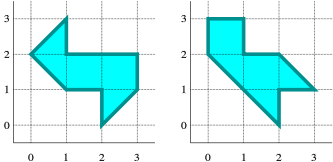
\includegraphics[scale=0.5]{drums.png}    
  \end{center}
\caption{Deux images renvoyant des sons identiques (source : Wikipédia)}
\label{drum}
\end{figure}
%#############################################################################################################%
%#############################################################################################################%
%#############################################################################################################%

\section*{Bonus}

Nous avons essayé de reconstruire un son à partir des valeurs propres du Laplacien de Dirichlet. Pour cela, à partir du spectre des valeurs propres $\{\lambda_1, \lambda_2, ...\}$ de l'image, on en déduit les fréquences pouvant se propager dans la cavité définie par l'image, de la forme $\{\alpha \sqrt{\lambda_1}, \alpha \sqrt{\lambda_2}, ...\}$, $\alpha$ étant une constante choisie de façon à ce que le spectre obtenu soit compris entre 100Hz et 2kHz.

En pratique, $\alpha = 40$ et on ne retient que 3 valeurs propres. On associe la même puissance à chacune des 3 fréquences calculées. On peut changer ces différents paramètres pour entendre des sons différents.

Afin d'entendre le son associé à l'image \texttt{beetle-11.pgm} par exemple, entrer : 
\begin{center}
  \texttt{./sound.sh database/beetle-11.pgm}
\end{center}

Nous avons également développé un petit jeu qui consiste à retrouver parmi les sons de plusieurs objets celui appartenant à la même catégorie qu'un motif de départ. 
Il est accessible par :
\begin{center}
  \texttt{./sound\_game.sh}
\end{center}

%#############################################################################################################%
%#############################################################################################################%
%#############################################################################################################%

\bibliographystyle{alpha}
\bibliography{Biblio}
\nocite{*}

\end{document}